\documentclass[11pt,a4paper]{article}

\usepackage[T1]{fontenc}
\usepackage[utf8]{inputenc}
\usepackage[margin=25mm]{geometry}
\usepackage{amsmath,amssymb}
\usepackage{graphicx}
\usepackage{booktabs}
\usepackage{tabularx}
\usepackage{tikz}
\usepackage{pgfplots}
\pgfplotsset{compat=1.16}
\usetikzlibrary{arrows.meta,patterns}
\usepackage[hidelinks]{hyperref}
\usepackage{siunitx}
\sisetup{detect-all}

\title{Dead Time in Voltage Source Converters:\\
Symmetric and Asymmetric Insertion, Harmonic Effects\\
(with Emphasis on Even Harmonics) and Compensation Methods}
\author{}
\date{}

\begin{document}
\maketitle

\begin{abstract}
Dead time (blanking time) is the deliberate delay inserted between the turn-off of one
switch of a phase leg and the turn-on of its complementary switch, and it is unavoidable
in hard-switched voltage source converters (VSCs). Although it is a small fraction of the
switching period, it introduces a systematic volt--second error that distorts the output
voltage. This note reviews the origin of the error, the difference between symmetric and
asymmetric dead-time insertion, and the resulting harmonic spectrum. Particular attention
is given to the mechanisms that break the half-wave symmetry of the error voltage and
therefore generate \emph{even} harmonics and a DC component --- effects that are often
overlooked because the textbook analysis predicts odd harmonics only. Hardware and
software compensation strategies are then surveyed at a system level, without entering
into implementation details, and a comparison is given to support the selection of a
suitable method. A comprehensive bibliography is provided.
\end{abstract}

\tableofcontents

\section{Introduction}

In a hard-switched phase leg the two series-connected devices must never conduct
simultaneously. Because turn-off is always slower than turn-on for minority-carrier
devices, and because gate-driver propagation delays are not perfectly matched, a blanking
interval $T_d$ is inserted between the two gate commands. The interval must cover the
worst-case turn-off storage and fall time, the spread of the driver propagation delays,
and the tolerance of the modulator, over the full temperature and current range
\cite{holmes2003,mohan2003,wintrich2015}.

During this interval both devices are off and the leg output potential is not imposed by
the modulator: it is determined by the sign of the load current, which freewheels through
one of the antiparallel diodes. The resulting output voltage therefore differs from the
commanded one by a pulse of amplitude equal to the DC-link voltage and duration equal to
the dead time. Averaged over one modulation period, this becomes a current-polarity
dependent voltage error that produces low-order harmonic distortion, torque ripple in
motor drives, current distortion in grid-tied converters, and --- at low modulation index
--- gain loss and even instability of the current loop
\cite{murai1987,jeong1991,dodson1990,guha2018}.

The classical treatment assumes that the error voltage is a square wave in phase with the
load current and concludes that only odd harmonics ($5$th, $7$th, $11$th, $13$th, \dots)
are produced. This conclusion holds only if the error waveform has half-wave symmetry.
Several practical mechanisms destroy that symmetry, and the consequence is the appearance
of even harmonics and of a DC component, which are far more troublesome than the odd ones
because of transformer saturation, DC injection limits, and low-frequency torque
pulsation. Section~\ref{sec:even} is devoted to this point.

\section{Dead-time insertion strategies}

\subsection{Nominal, effective and equivalent dead time}

Let $T_d$ be the nominal blanking time programmed in the modulator, $t_{on}$ the turn-on
delay (including driver propagation and current rise) and $t_{off}$ the turn-off delay
(including storage time and voltage rise). The volt--second error does not depend on
$T_d$ alone but on the \emph{effective} dead time
\begin{equation}
T_{d}^{\,\mathrm{eff}} \;=\; T_d + t_{on} - t_{off} ,
\label{eq:teff}
\end{equation}
which can be significantly larger or smaller than $T_d$ and, for IGBTs, is strongly
dependent on collector current and junction temperature
\cite{jeong1991,choi1996,munoz1999,bedetti2015}. Because $t_{on}$ and $t_{off}$ of the
upper and lower device are never identical --- different gate resistors, different layout,
different thermal state, device-to-device spread --- the effective dead time of the
positive-current commutation generally differs from that of the negative-current
commutation:
\begin{equation}
T_{d}^{+} \neq T_{d}^{-} .
\end{equation}
This is the first source of asymmetry, and it exists even when the modulator inserts a
perfectly symmetric blanking time.

\subsection{Symmetric versus asymmetric insertion}

Two implementations are commonly found in modulators (Fig.~\ref{fig:timing}):

\begin{itemize}
\item \textbf{Symmetric insertion.} The rising edge of each of the two complementary gate
signals is delayed by $T_d/2$ (or the pulse of each device is shortened by $T_d/2$ at both
edges). The commanded pulse remains centred on the carrier reference; the modulation is
unbiased in time but each pulse is shortened by $T_d$.
\item \textbf{Asymmetric (one-edge) insertion.} The whole delay $T_d$ is applied to the
turn-on edge only, or is applied to one device only. The pulse centroid is displaced by
$T_d/2$, which introduces an additional phase shift of the fundamental and, more
importantly, an upper/lower asymmetry of the leg behaviour.
\end{itemize}

A further, often unintentional, source of asymmetry is the combination of the blanking
logic with the sampling scheme: single-update (symmetric) versus double-update
(asymmetric) regular sampling produces different residual errors, and asymmetric regular
sampling introduces a sideband structure of its own \cite{holmes2003,oliveira2007}.

From the point of view of the harmonic content, what matters is not the label attached to
the insertion scheme but whether the resulting volt--second error is the same, in
magnitude and duration, for the two half-cycles of the load current.

\begin{figure}[htb]
\centering
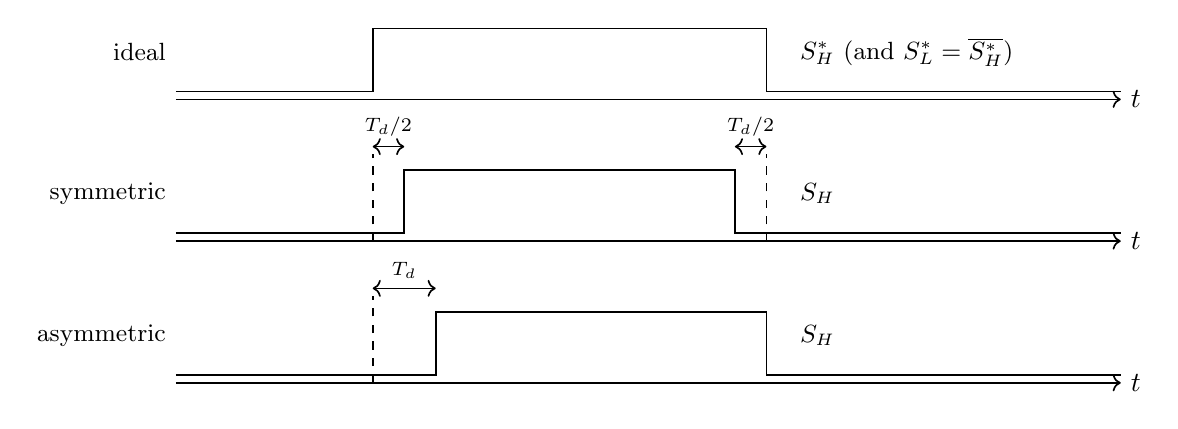
\begin{tikzpicture}[x=1mm,y=1mm,line width=0.6pt]
% reference pulse
\draw[->] (0,44) -- (120,44) node[right]{$t$};
\node[left] at (0,50) {\small ideal};
\draw (0,45) -- (25,45) -- (25,53) -- (75,53) -- (75,45) -- (120,45);
\node[right] at (78,50) {\small $S_H^{*}$ (and $S_L^{*}=\overline{S_H^{*}}$)};

% symmetric
\draw[->] (0,26) -- (120,26) node[right]{$t$};
\node[left] at (0,32) {\small symmetric};
\draw (0,27) -- (29,27) -- (29,35) -- (71,35) -- (71,27) -- (120,27);
\draw[dashed] (25,26) -- (25,37);
\draw[dashed] (75,26) -- (75,37);
\draw[<->] (25,38) -- (29,38);
\node[above] at (27,38) {\scriptsize $T_d/2$};
\draw[<->] (71,38) -- (75,38);
\node[above] at (73,38) {\scriptsize $T_d/2$};
\node[right] at (78,32) {\small $S_H$};

% asymmetric
\draw[->] (0,8) -- (120,8) node[right]{$t$};
\node[left] at (0,14) {\small asymmetric};
\draw (0,9) -- (33,9) -- (33,17) -- (75,17) -- (75,9) -- (120,9);
\draw[dashed] (25,8) -- (25,19);
\draw[<->] (25,20) -- (33,20);
\node[above] at (29,20) {\scriptsize $T_d$};
\node[right] at (78,14) {\small $S_H$};
\end{tikzpicture}
\caption{Symmetric (both edges shifted by $T_d/2$) versus asymmetric (turn-on edge only
delayed by $T_d$) dead-time insertion. In both cases the on-pulse is shortened by $T_d$,
but in the asymmetric case its centroid is displaced.}
\label{fig:timing}
\end{figure}

\section{Average voltage error model}

\subsection{Dead-time term}

Assume the load current $i$ is approximately constant over one switching period $T_s$ and
that the leg output is clamped by the freewheeling diode during the blanking interval.
The average error between the actual and the commanded leg voltage is
\begin{equation}
\Delta v \;=\; -\,\mathrm{sgn}(i)\;\frac{T_{d}^{\,\mathrm{eff}}}{T_s}\,V_{dc}
\;\triangleq\; -\,\mathrm{sgn}(i)\,V_{\!\varepsilon} ,
\label{eq:verr}
\end{equation}
i.e.\ the converter loses voltage when it sources current and gains voltage when it sinks
it \cite{jeong1991,choi1996,munoz1999}. With $T_d = \SI{3}{\micro\second}$,
$f_s = \SI{4}{\kilo\hertz}$ and $V_{dc} = \SI{700}{\volt}$ the error is about
\SI{8.4}{\volt} per leg, i.e.\ some \SI{2}{\percent} of the fundamental at rated voltage
but a much larger relative error at low speed or low modulation index.

If the two half-cycles see different effective dead times, \eqref{eq:verr} becomes
\begin{equation}
\Delta v \;=\;
\begin{cases}
-V_{\!\varepsilon}^{+}, & i>0\\[2pt]
+V_{\!\varepsilon}^{-}, & i<0 .
\end{cases}
\label{eq:verrasym}
\end{equation}

\subsection{Conduction-drop term}

The on-state voltage drops of the transistor ($V_{ce}$ or $R_{ds}i$) and of the diode
($V_{f}$) add a second error term. For $i>0$, with duty ratio $d$ of the upper device,
\begin{equation}
\Delta v_{cond} \;=\; -\Big[\,d\,V_{ce} + (1-d)\,V_{f}\Big]
\;=\; -\left[\frac{V_{ce}+V_{f}}{2} + \frac{V_{ce}-V_{f}}{2}\,(2d-1)\right],
\label{eq:vcond}
\end{equation}
and the sign reverses for $i<0$. The first term behaves like the dead-time term (a square
wave in phase with the current); the second is proportional to the product of
$\mathrm{sgn}(i)$ and the modulating function $(2d-1)\simeq m\sin\omega t$, and this
product is the key to the even-harmonic generation discussed in
Section~\ref{sec:even}. Note that in wide-bandgap converters the reverse-conduction drop
during the dead time can be very large (\SIrange{3}{5}{\volt} for a GaN HEMT in third
quadrant without a gate signal), which makes this term comparable with the dead-time term
itself \cite{lidow2019,zhang2015}.

\subsection{Zero-current clamping and parasitic capacitances}

Around the current zero crossing the ideal model fails. When $|i|$ is smaller than the
ripple, the current changes sign within the switching period and the polarity-dependent
error becomes ambiguous; furthermore, if the current is not sufficient to charge and
discharge the device output capacitances within the blanking interval, the leg output
voltage does not commutate at all and remains clamped at its previous value
(zero-current-clamping, ZCC). The result is a flat region of several degrees around the
zero crossing in which the voltage error is not a square wave but a smooth,
current-dependent function \cite{benbrahim2004,zhang2014,park2012}. The width of this
region is not the same for the two crossings when the leg is thermally or electrically
asymmetric, which is yet another source of even harmonics.

\section{Harmonic content: the symmetric case}

Consider a sinusoidal current $i=\hat{I}\sin(\omega t-\varphi)$ and a perfectly symmetric
leg, $V_{\!\varepsilon}^{+} = V_{\!\varepsilon}^{-} = V_{\!\varepsilon}$. The error
voltage is a square wave of amplitude $V_{\!\varepsilon}$, synchronous with the current
and phase-shifted by $\varphi$ with respect to the voltage:
\begin{equation}
\Delta v(t) \;=\; -\frac{4V_{\!\varepsilon}}{\pi}
\sum_{n=1,3,5,\dots} \frac{1}{n}\,\sin\!\big[n(\omega t-\varphi)\big].
\label{eq:square}
\end{equation}
The waveform has half-wave symmetry, $\Delta v(t+T/2) = -\Delta v(t)$, hence
\emph{only odd harmonics} are present, with amplitudes decaying as $1/n$. In a balanced
three-phase three-wire system the triplen components are zero-sequence and do not drive
current, so the dominant terms are the $5$th, $7$th, $11$th, $13$th, which appear as
$6k$ torque ripple in a machine and as characteristic low-order distortion in a grid-tied
converter \cite{jeong1991,choi1996,leggate1997,holmes2003}.

It is worth stressing an intermediate case. If the two half-cycles differ only in
\emph{amplitude} but not in \emph{duration}, \eqref{eq:verrasym} can be rewritten as
\begin{equation}
\Delta v(t) \;=\; -\underbrace{\frac{V_{\!\varepsilon}^{+}-V_{\!\varepsilon}^{-}}{2}}_{\text{DC}}
\;-\;\underbrace{\frac{V_{\!\varepsilon}^{+}+V_{\!\varepsilon}^{-}}{2}}_{\text{amplitude}}
\cdot \mathrm{sq}(\omega t - \varphi),
\label{eq:amplasym}
\end{equation}
i.e.\ an unbalanced amplitude produces a \emph{DC offset plus odd harmonics}, but no even
harmonics by itself. This is an important distinction: amplitude asymmetry alone is not
sufficient to generate even orders; it is however sufficient to generate a DC voltage
error, which then closes a feedback loop that does generate them.

\section{Mechanisms generating even harmonics and DC}
\label{sec:even}

Even harmonics require the loss of half-wave symmetry in a stricter sense: the positive
and negative intervals of the error waveform must have \emph{different durations}, or the
error must contain a term modulated by the fundamental itself. Four practical mechanisms
are relevant.

\subsection{Displacement of the current zero crossings}

Let the positive interval of $\mathrm{sgn}(i)$ last $\pi+\delta$ instead of $\pi$, i.e.\
duty ratio $D = \tfrac{1}{2} + \tfrac{\delta}{2\pi}$. The Fourier coefficients of a
$\pm 1$ wave with duty ratio $D$ are
\begin{equation}
c_0 = 2D-1, \qquad
|c_n| = \frac{4}{n\pi}\,\big|\sin(n\pi D)\big| ,
\label{eq:dutyfourier}
\end{equation}
so that for a small displacement $\delta$
\begin{equation}
c_0 \simeq \frac{\delta}{\pi}\,V_{\!\varepsilon}, \qquad
|c_{n,\text{even}}| \simeq \frac{2\delta}{\pi}\,V_{\!\varepsilon}
\quad (n=2,4,6,\dots \text{ small}),
\end{equation}
i.e.\ each low-order even harmonic is approximately \emph{twice} the DC term and, unlike
the odd ones, its amplitude does not decay as $1/n$ for the first few orders
(Fig.~\ref{fig:spectrum}). A zero-crossing displacement of only $\SI{7}{\degree}$ already
produces even harmonics of about \SI{6}{\percent} of the fundamental error component.

The zero crossings are displaced whenever the load current contains a DC offset --- from
current-sensor offset or gain mismatch, from ADC offset, from an unbalanced modulator, or
from a previous transient. This creates a \emph{positive feedback loop}: the DC current
offset displaces the crossings, the displacement produces a DC voltage error, and the DC
voltage error drives further DC current through the small loop resistance. In
transformer-coupled or transformerless grid-tied converters this mechanism is a
well-documented cause of DC injection, transformer saturation and second-harmonic
distortion \cite{buticchi2011,buticchi2013,sharma2005,armstrong2006,blaabjerg2006}.

\subsection{Interaction between conduction drops and the modulating function}

The second term of \eqref{eq:vcond} is proportional to
$\mathrm{sgn}(i)\cdot m\sin\omega t$. The product of two waveforms of odd harmonic
content yields even orders and a DC component:
\begin{equation}
\mathrm{sq}(\omega t-\varphi)\cdot m\sin(\omega t)
\;=\; \frac{2m}{\pi}\cos\varphi
\;-\;\frac{2m}{\pi}\cos(2\omega t-\varphi) + \dots
\end{equation}
Hence a transistor/diode drop mismatch $\left(V_{ce}-V_{f}\right)$ generates a DC term and
a second harmonic of comparable magnitude,
$\approx \tfrac{m}{\pi}\left(V_{ce}-V_{f}\right)$, \emph{even with a perfectly symmetric
dead time and no current offset}. With $V_{ce}-V_{f}\approx\SI{0.5}{\volt}$ this is of the
order of \SI{0.16}{\volt} per leg: negligible at rated voltage, but comparable with the
fundamental command at very low speed, and directly relevant for GaN-based converters
where the third-quadrant drop is several volts \cite{munoz1999,bedetti2015,lidow2019}.

\subsection{Upper/lower asymmetry combined with modulation}

When $T_{d}^{+}\neq T_{d}^{-}$ (mismatched gate resistors, unequal driver delays,
different junction temperatures of the upper and lower device, one-edge dead-time
insertion), the DC term of \eqref{eq:amplasym} appears immediately. In a closed-loop
drive the current controller reacts to it by biasing the modulating signal, which again
multiplies a fundamental-frequency quantity by $\mathrm{sgn}(i)$ and produces even orders.
In an open-loop V/f drive the DC voltage error directly produces a DC current, closing the
same loop described above. Asymmetric leg cooling --- very common in half-bridge modules
with a hot upper device --- makes this effect load- and time-dependent.

\subsection{Asymmetric zero-current clamping and single-phase operation}

The ZCC region described above is generally not symmetric about the two crossings, since
the charge required to commutate the leg and the available current differ for the two
transitions; the resulting error waveform has different positive and negative durations,
producing even orders \cite{benbrahim2004,zhang2014}. In single-phase converters (and in
three-phase converters with an unbalanced or four-wire load) there is no cancellation
mechanism, so the DC and even components appear directly in the output current
\cite{buticchi2011,herran2013}.

\begin{figure}[htb]
\centering
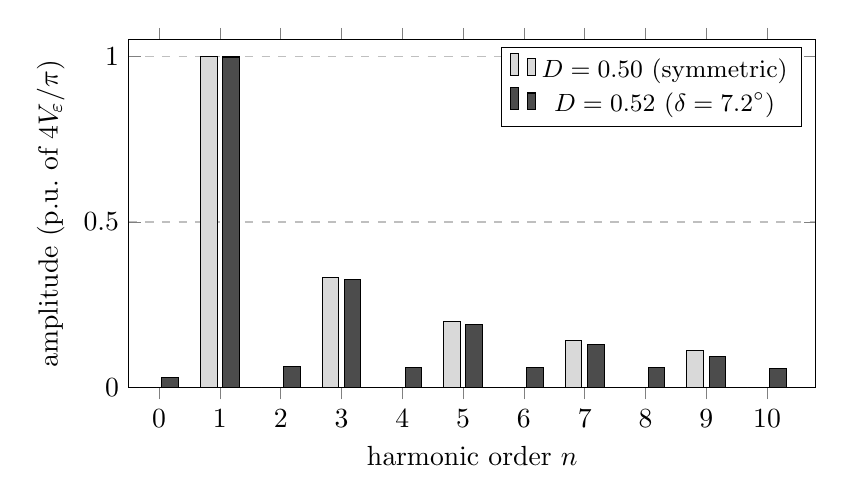
\begin{tikzpicture}
\begin{axis}[
  width=0.85\textwidth, height=6cm,
  ybar, bar width=6pt,
  xlabel={harmonic order $n$}, ylabel={amplitude (p.u.\ of $4V_{\!\varepsilon}/\pi$)},
  xmin=-0.5, xmax=10.8, ymin=0, ymax=1.05,
  xtick={0,1,2,3,4,5,6,7,8,9,10},
  legend style={at={(0.98,0.98)},anchor=north east,font=\small},
  ymajorgrids=true, grid style=dashed,
]
\addplot[fill=gray!30,draw=black] coordinates
 {(0,0) (1,1.0) (2,0) (3,0.3333) (4,0) (5,0.2) (6,0) (7,0.1429) (8,0) (9,0.1111) (10,0)};
\addlegendentry{$D=0.50$ (symmetric)}
\addplot[fill=black!70,draw=black] coordinates
 {(0,0.0314) (1,0.9980) (2,0.0627) (3,0.3274) (4,0.0622) (5,0.1902) (6,0.0613) (7,0.1293) (8,0.0602) (9,0.0938) (10,0.0587)};
\addlegendentry{$D=0.52$ ($\delta=\SI{7.2}{\degree}$)}
\end{axis}
\end{tikzpicture}
\caption{Spectrum of the dead-time error voltage for a symmetric error square wave and for
an error wave whose zero crossings are displaced by $\SI{7.2}{\degree}$. The displacement
introduces a DC component and even harmonics of nearly constant amplitude, at the expense
of a barely visible change of the odd orders.}
\label{fig:spectrum}
\end{figure}

\subsection{Sequence components and system consequences}

In a balanced three-phase converter with identical legs, the harmonic sets of the error
voltage have the following sequences: the DC component is zero-sequence (no current in a
three-wire system, but a real DC magnetising bias if a transformer is present with a
neutral path or in single-phase legs); the $2$nd harmonic is \emph{negative} sequence and
therefore does drive current in a three-wire system; the $4$th is positive sequence; the
$6$th is zero sequence. Consequences:

\begin{itemize}
\item \textbf{Machine drives.} The $2$nd harmonic (negative sequence) maps into a
$3\omega$ torque ripple in the rotor frame, while a DC current component produces a
$1\omega$ ripple and a localised heating of one phase; the classical $5$th/$7$th pair
gives the well-known $6\omega$ ripple \cite{sukegawa1991,kim2003,kim2010}.
\item \textbf{Grid-tied converters.} DC injection is limited by grid codes and product
standards (typically \SI{0.5}{\percent} of rated current or less), and even harmonics are
limited more severely than odd ones --- IEEE Std~519 restricts them to \SI{25}{\percent}
of the adjacent odd limits \cite{ieee519,iec61000_3_2,iec61727,ieee1547}. A DC bias
saturates distribution transformers, increases their losses and noise, and further
distorts the current \cite{buticchi2013}.
\item \textbf{DC-link and stability.} The distortion reflects into the DC-link current and
interacts with the input filter, degrading damping and, at light load, causing
low-frequency instability \cite{guha2018}.
\end{itemize}

\section{Hardware compensation and mitigation}

The hardware approach either reduces the required dead time or removes its effect at the
commutation itself.

\begin{itemize}
\item \textbf{Matched and optimised gate drives.} Reducing the spread of $t_{on}$ and
$t_{off}$ between the two devices allows a shorter $T_d$ with the same margin, and reduces
the upper/lower asymmetry that generates DC and even orders. Negative gate bias, active
Miller clamping and low-inductance layout suppress the cross-talk that would otherwise
force a longer blanking time \cite{zhang2015,wintrich2015}.
\item \textbf{Adaptive (self-adjusting) dead time.} The blanking interval is terminated as
soon as the commutation is actually complete, detected through the collector--emitter (or
drain--source) voltage, the $dv/dt$, or the desaturation comparator. The dead time then
tracks the operating point instead of being set by the worst case
\cite{chen2008,lin2009,park2012}.
\item \textbf{Current-polarity-based gating (dead-time elimination).} If the sign of the
leg current is known, only the device that must actually conduct is gated and the
complementary one is kept permanently off; the freewheeling diode takes the current and no
blanking interval is needed. A hysteresis band or a hybrid strategy is required around the
zero crossing \cite{chen2008,lin2009,wang2011}.
\item \textbf{Soft-switching topologies.} In ZVS resonant-pole and auxiliary resonant
commutated pole (ARCP) legs the output transition is imposed by the resonant network
rather than by the device gating, and the dead-time distortion is largely removed at the
price of an auxiliary circuit \cite{devoncy1990,mcmurray1989}.
\item \textbf{Snubber and $C_{oss}$ shaping.} Capacitive snubbers linearise the transition
during the blanking interval; the voltage error becomes a smooth function of the current
rather than a hard pulse, but the zero-crossing clamping region widens
\cite{zhang2014}.
\item \textbf{Fast wide-bandgap devices.} SiC and GaN allow dead times of tens of
nanoseconds, so that $T_d/T_s$ --- and with it the whole distortion --- is reduced by one
or two orders of magnitude even at high switching frequency. Care is needed because the
reverse-conduction drop during the dead time is high, making the residual error dependent
on the dead time in a stronger, non-linear way \cite{lidow2019,zhang2015}.
\item \textbf{Analog pulse-correction circuits.} Historically, the missing volt--seconds
were restored by hardware that lengthened the following pulse according to the detected
current polarity \cite{murai1987,dodson1990}.
\end{itemize}

\section{Software compensation}

Software methods do not remove the error at the leg; they add a corrective term to the
modulator reference so that the \emph{average} output matches the command.

\begin{itemize}
\item \textbf{Average feed-forward compensation.} The simplest and most widespread scheme
adds $+\mathrm{sgn}(i)\,V_{\!\varepsilon}$ to the voltage reference of each phase. It
requires only the current sign and a value of $V_{\!\varepsilon}$; its weakness is
precisely the sign detection near the zero crossings, where noise and ripple cause
chattering \cite{jeong1991,choi1995,choi1996,sukegawa1991}.
\item \textbf{Improved polarity detection.} Hysteresis bands, use of the current
\emph{reference} instead of the measurement, use of an observed/estimated current, and
smooth (piecewise-linear or arctangent) transition functions across the crossing reduce
the residual distortion and, importantly, avoid introducing an artificial asymmetry
between the two crossings \cite{benbrahim2004,urasaki2005,hwang2010}.
\item \textbf{Pulse-based compensation.} Instead of a mean value, each individual PWM
pulse is corrected, which is more accurate at high switching frequency and short pulse
widths and handles the minimum-pulse limitation explicitly
\cite{leggate1997,oliveira2007}.
\item \textbf{Look-up tables and self-commissioning.} The complete inverter non-linearity
(dead time, conduction drops, clamping) is identified as a single current-dependent
voltage curve, obtained by a standstill test or by online regression, and stored in a
table. This captures the asymmetric part of the characteristic and is therefore effective
against DC and even harmonics \cite{pellegrino2010,bedetti2015,cichowski2005}.
\item \textbf{Disturbance observers and model-based estimation.} The distortion is treated
as an unknown disturbance in the stationary or synchronous frame and estimated by an
observer, then cancelled. No explicit dead-time model is needed
\cite{kim2003,kim2010,munoz1999}.
\item \textbf{Closed-loop harmonic regulators.} Proportional-resonant and
vector-proportional-integral regulators tuned at the offending frequencies, multiple
synchronous reference frames, repetitive control and iterative learning control suppress
whatever periodic distortion is present, provided the loop bandwidth is sufficient. For
even harmonics the resonant terms must be placed at $2\omega$ and $4\omega$ --- in the
synchronous frame at $\omega$ and $3\omega$ --- which is often forgotten when only the
$6k$ terms are addressed \cite{teodorescu2006,zhou2003,lascu2007,yepes2011}.
\item \textbf{Explicit DC-component control.} A dedicated slow integral loop acting on the
measured DC content of each phase current (or on an estimate of the transformer flux bias)
breaks the positive feedback described in Section~\ref{sec:even} and is the most direct
remedy for DC injection and second-harmonic distortion
\cite{buticchi2011,buticchi2013,armstrong2006}.
\item \textbf{Modulation-level remedies.} Mixed or hybrid PWM strategies, clamping of the
leg carrying the largest current, and per-leg dead-time elimination based on the reference
current sign reduce the number of commutations affected by the blanking time
\cite{wang2011,chen2008}.
\item \textbf{Adaptive and learning schemes.} Recursive least squares, multiple linear
regression on a physical model, and neural-network estimators adapt the compensation to
temperature and ageing, which is relevant because $T_{d}^{\,\mathrm{eff}}$ drifts with the
junction temperature \cite{urasaki2005,bedetti2015,herran2013}.
\end{itemize}

A practical remark: any compensation scheme that applies the \emph{same} correction to the
two half-cycles cannot remove the DC and even-harmonic content produced by an asymmetric
leg. Two separate compensation values, or a closed-loop DC regulator, are required.

\begin{table}[htb]
\centering
\caption{Qualitative comparison of the main compensation approaches.}
\label{tab:comparison}
\small
\begin{tabularx}{\textwidth}{@{}lXccc@{}}
\toprule
Method & Principle & Extra HW & Needs $\mathrm{sgn}(i)$ & Removes DC/even \\
\midrule
Matched drivers, short $T_d$ & reduce the cause & no & no & partly \\
Adaptive dead time & terminate blanking on $dv/dt$ & yes & no & yes \\
Polarity-based gating & no blanking at all & yes & yes & partly \\
Soft switching (ARCP) & resonant transition & yes & no & yes \\
Average feed-forward & add $V_{\!\varepsilon}\,\mathrm{sgn}(i)$ & no & yes & no \\
Pulse-based correction & per-pulse volt--second restore & no & yes & no \\
LUT / self-commissioning & identified non-linearity curve & no & yes & yes \\
Disturbance observer & estimate and cancel & no & no & yes \\
Resonant / repetitive control & closed-loop harmonic rejection & no & no & yes (if tuned) \\
Explicit DC loop & regulate DC current to zero & no & no & yes (DC only) \\
\bottomrule
\end{tabularx}
\end{table}

\section{Practical guidelines}

\begin{enumerate}
\item Size $T_d$ on the worst case of turn-off delay and driver spread, but re-verify it
at rated temperature: an unnecessarily conservative dead time is paid for at every
switching event.
\item Characterise $T_{d}^{\,\mathrm{eff}}$ rather than $T_d$; measure it, if possible, as
the offset of the voltage/current characteristic at standstill.
\item Verify separately the two half-cycles. A spectrum showing $2$nd and $4$th harmonics
or a DC component is a symptom of leg asymmetry, sensor offset or asymmetric clamping ---
not of the dead time as such.
\item Check current sensor offset and gain matching before blaming the modulator: the two
effects are indistinguishable in the spectrum, and they reinforce each other.
\item Use a weighted THD (WTHD) or the individual low-order limits of the applicable
standard, not the plain THD, to judge the residual distortion \cite{holmes2003,ieee519}.
\item Combine a feed-forward term (fast, coarse) with a closed-loop harmonic or DC
regulator (slow, accurate): the first handles the transient behaviour, the second removes
the residual asymmetric content.
\end{enumerate}

\section{Conclusion}

Dead time is a small quantity with a disproportionate effect on the low-frequency spectrum
of a voltage source converter. The classical model, based on a symmetric error square wave
synchronous with the load current, explains the $5$th, $7$th, $11$th and $13$th harmonics
and the associated $6\omega$ torque ripple. It does not explain the DC component and the
even harmonics that are routinely observed on real converters. These arise when the
half-wave symmetry of the error waveform is broken --- by displaced current zero crossings
(sensor offset or DC current), by the interaction between the transistor/diode drop
mismatch and the modulating function, by unequal effective dead times of the upper and
lower device, or by asymmetric zero-current clamping. Because even harmonics and DC are
constrained much more tightly than odd harmonics, and because they feed back on themselves
through the load, they deserve explicit attention. Hardware measures act on the cause
(shorter and adaptive dead time, polarity-based gating, soft switching, wide-bandgap
devices); software measures act on the effect (feed-forward, identified non-linearity
tables, observers, resonant and repetitive control, dedicated DC loops). The two families
are complementary, and only the methods that treat the two half-cycles independently are
effective against the asymmetric part of the distortion.

\begin{thebibliography}{99}
\sloppy

\bibitem{holmes2003}
D.~G. Holmes and T.~A. Lipo, \emph{Pulse Width Modulation for Power Converters:
Principles and Practice}. Piscataway, NJ, USA: IEEE Press/Wiley, 2003.

\bibitem{mohan2003}
N.~Mohan, T.~M. Undeland, and W.~P. Robbins, \emph{Power Electronics: Converters,
Applications and Design}, 3rd ed. New York, NY, USA: Wiley, 2003.

\bibitem{wintrich2015}
A.~Wintrich, U.~Nicolai, W.~Tursky, and T.~Reimann, \emph{Application Manual Power
Semiconductors}, 2nd ed. Ilmenau, Germany: SEMIKRON/ISLE, 2015.

\bibitem{murai1987}
Y.~Murai, T.~Watanabe, and H.~Iwasaki, ``Waveform distortion and correction circuit for
PWM inverters with switching lag-times,'' \emph{IEEE Trans. Ind. Appl.}, vol.~IA-23,
no.~5, pp.~881--886, Sep. 1987.

\bibitem{dodson1990}
R.~C. Dodson, P.~D. Evans, H.~T. Yazdi, and S.~C. Harley, ``Compensating for dead time
degradation of PWM inverter waveforms,'' \emph{IEE Proc. B}, vol.~137, no.~2,
pp.~73--81, Mar. 1990.

\bibitem{jeong1991}
S.-G. Jeong and M.-H. Park, ``The analysis and compensation of dead-time effects in PWM
inverters,'' \emph{IEEE Trans. Ind. Electron.}, vol.~38, no.~2, pp.~108--114, Apr. 1991.

\bibitem{sukegawa1991}
T.~Sukegawa, K.~Kamiyama, K.~Mizuno, T.~Matsui, and T.~Okuyama, ``Fully digital,
vector-controlled PWM VSI-fed AC drives with an inverter dead-time compensation
strategy,'' \emph{IEEE Trans. Ind. Appl.}, vol.~27, no.~3, pp.~552--559, May/Jun. 1991.

\bibitem{choi1995}
J.-W. Choi and S.-K. Sul, ``A new compensation strategy reducing voltage/current
distortion in PWM VSI systems operating with low output voltages,'' \emph{IEEE Trans.
Ind. Appl.}, vol.~31, no.~5, pp.~1001--1008, Sep./Oct. 1995.

\bibitem{choi1996}
J.-W. Choi and S.-K. Sul, ``Inverter output voltage synthesis using novel dead time
compensation,'' \emph{IEEE Trans. Power Electron.}, vol.~11, no.~2, pp.~221--227,
Mar. 1996.

\bibitem{leggate1997}
D.~Leggate and R.~J. Kerkman, ``Pulse-based dead-time compensator for PWM voltage
inverters,'' \emph{IEEE Trans. Ind. Electron.}, vol.~44, no.~2, pp.~191--197, Apr. 1997.

\bibitem{munoz1999}
A.~R. Mu\~{n}oz and T.~A. Lipo, ``On-line dead-time compensation technique for open-loop
PWM-VSI drives,'' \emph{IEEE Trans. Power Electron.}, vol.~14, no.~4, pp.~683--689,
Jul. 1999.

\bibitem{kim2003}
H.-S. Kim, H.-T. Moon, and M.-J. Youn, ``On-line dead-time compensation method using
disturbance observer,'' \emph{IEEE Trans. Power Electron.}, vol.~18, no.~6,
pp.~1336--1345, Nov. 2003.

\bibitem{benbrahim2004}
L.~Ben-Brahim, ``On the compensation of dead time and zero-current crossing for a
PWM-inverter-controlled AC servo drive,'' \emph{IEEE Trans. Ind. Electron.}, vol.~51,
no.~5, pp.~1113--1118, Oct. 2004.

\bibitem{cichowski2005}
A.~Cichowski and J.~Nieznanski, ``Self-tuning dead-time compensation method for
voltage-source inverters,'' \emph{IEEE Power Electron. Lett.}, vol.~3, no.~2,
pp.~72--75, Jun. 2005.

\bibitem{urasaki2005}
N.~Urasaki, T.~Senjyu, K.~Uezato, and T.~Funabashi, ``An adaptive dead-time compensation
strategy for voltage source inverter fed motor drives,'' \emph{IEEE Trans. Power
Electron.}, vol.~20, no.~5, pp.~1150--1160, Sep. 2005.

\bibitem{oliveira2007}
A.~C. Oliveira, C.~B. Jacobina, and A.~M.~N. Lima, ``Improved dead-time compensation for
sinusoidal PWM inverters operating at high switching frequencies,'' \emph{IEEE Trans.
Ind. Electron.}, vol.~54, no.~4, pp.~2295--2304, Aug. 2007.

\bibitem{chen2008}
L.~Chen and F.~Z. Peng, ``Dead-time elimination for voltage source inverters,''
\emph{IEEE Trans. Power Electron.}, vol.~23, no.~2, pp.~574--580, Mar. 2008.

\bibitem{lin2009}
Y.-K. Lin and Y.-S. Lai, ``Dead-time elimination of PWM-controlled inverter/converter
without separate power sources for current polarity detection circuit,'' \emph{IEEE
Trans. Ind. Electron.}, vol.~56, no.~6, pp.~2121--2127, Jun. 2009.

\bibitem{hwang2010}
S.-H. Hwang and J.-M. Kim, ``Dead time compensation method for voltage-fed PWM
inverter,'' \emph{IEEE Trans. Energy Convers.}, vol.~25, no.~1, pp.~1--10, Mar. 2010.

\bibitem{kim2010}
S.-Y. Kim, W.~Lee, M.-S. Rho, and S.-Y. Park, ``Effective dead-time compensation using a
simple vectorial disturbance estimator in PMSM drives,'' \emph{IEEE Trans. Ind.
Electron.}, vol.~57, no.~5, pp.~1609--1614, May 2010.

\bibitem{pellegrino2010}
G.~Pellegrino, P.~Guglielmi, E.~Armando, and R.~I. Bojoi, ``Self-commissioning algorithm
for inverter non-linearity compensation in sensorless induction motor drives,''
\emph{IEEE Trans. Ind. Appl.}, vol.~46, no.~4, pp.~1416--1424, Jul./Aug. 2010.

\bibitem{wang2011}
Y.~Wang, Q.~Gao, and X.~Cai, ``Mixed PWM for dead-time elimination and compensation in a
grid-tied inverter,'' \emph{IEEE Trans. Ind. Electron.}, vol.~58, no.~10,
pp.~4797--4803, Oct. 2011.

\bibitem{park2012}
Y.~Park and S.-K. Sul, ``A novel method utilizing trapezoidal voltage to compensate for
inverter nonlinearity,'' \emph{IEEE Trans. Power Electron.}, vol.~27, no.~12,
pp.~4837--4846, Dec. 2012.

\bibitem{herran2013}
M.~A. Herr\'{a}n, J.~R. Fischer, S.~A. Gonz\'{a}lez, M.~G. Judewicz, and D.~O. Carrica,
``Adaptive dead-time compensation for grid-connected PWM inverters of single-stage PV
systems,'' \emph{IEEE Trans. Power Electron.}, vol.~28, no.~6, pp.~2816--2825,
Jun. 2013.

\bibitem{zhang2014}
Z.~Zhang and L.~Xu, ``Dead-time compensation of inverters considering snubber and
parasitic capacitance,'' \emph{IEEE Trans. Power Electron.}, vol.~29, no.~6,
pp.~3179--3187, Jun. 2014.

\bibitem{bedetti2015}
N.~Bedetti, S.~Calligaro, and R.~Petrella, ``Self-commissioning of inverter dead-time
compensation by multiple linear regression based on a physical model,'' \emph{IEEE Trans.
Ind. Appl.}, vol.~51, no.~5, pp.~3954--3964, Sep./Oct. 2015.

\bibitem{zhang2015}
Z.~Zhang, F.~Wang, L.~M. Tolbert, B.~J. Blalock, and D.~J. Costinett, ``Active gate
driver for fast switching and cross-talk suppression of SiC devices in a phase-leg
configuration,'' in \emph{Proc. IEEE Appl. Power Electron. Conf. (APEC)}, 2015,
pp.~774--781.

\bibitem{guha2018}
A.~Guha and G.~Narayanan, ``Impact of dead time on inverter input current, DC-link
dynamics, and light-load instability in rectifier-inverter-fed induction motor drives,''
\emph{IEEE Trans. Ind. Appl.}, vol.~54, no.~2, pp.~1414--1424, Mar./Apr. 2018.

\bibitem{lidow2019}
A.~Lidow, M.~de~Rooij, J.~Strydom, D.~Reusch, and J.~Glaser, \emph{GaN Transistors for
Efficient Power Conversion}, 3rd ed. Chichester, U.K.: Wiley, 2019.

\bibitem{mcmurray1989}
W.~McMurray, ``Resonant snubbers with auxiliary switches,'' in \emph{Conf. Rec. IEEE
Ind. Appl. Soc. Annu. Meeting}, 1989, pp.~289--834.

\bibitem{devoncy1990}
R.~W. De~Doncker and J.~P. Lyons, ``The auxiliary resonant commutated pole converter,''
in \emph{Conf. Rec. IEEE Ind. Appl. Soc. Annu. Meeting}, 1990, pp.~1228--1235.

\bibitem{teodorescu2006}
R.~Teodorescu, F.~Blaabjerg, M.~Liserre, and P.~C. Loh, ``Proportional-resonant
controllers and filters for grid-connected voltage-source converters,'' \emph{IEE Proc.
Electr. Power Appl.}, vol.~153, no.~5, pp.~750--762, Sep. 2006.

\bibitem{zhou2003}
K.~Zhou and D.~Wang, ``Digital repetitive controlled three-phase PWM rectifier,''
\emph{IEEE Trans. Power Electron.}, vol.~18, no.~1, pp.~309--316, Jan. 2003.

\bibitem{lascu2007}
C.~Lascu, L.~Asiminoaei, I.~Boldea, and F.~Blaabjerg, ``High performance current
controller for selective harmonic compensation in active power filters,'' \emph{IEEE
Trans. Power Electron.}, vol.~22, no.~5, pp.~1826--1835, Sep. 2007.

\bibitem{yepes2011}
A.~G. Yepes, F.~D. Freijedo, \'{O}.~L\'{o}pez, and J.~Doval-Gandoy, ``Analysis and design
of resonant current controllers for voltage-source converters by means of Nyquist
diagrams and sensitivity function,'' \emph{IEEE Trans. Ind. Electron.}, vol.~58, no.~11,
pp.~5231--5250, Nov. 2011.

\bibitem{buticchi2011}
G.~Buticchi, E.~Lorenzani, and G.~Franceschini, ``A DC offset current compensation
strategy in transformerless grid-connected power converters,'' \emph{IEEE Trans. Power
Del.}, vol.~26, no.~4, pp.~2743--2751, Oct. 2011.

\bibitem{buticchi2013}
G.~Buticchi and E.~Lorenzani, ``Detection method of the DC bias in distribution power
transformers,'' \emph{IEEE Trans. Ind. Electron.}, vol.~60, no.~8, pp.~3539--3549,
Aug. 2013.

\bibitem{armstrong2006}
M.~Armstrong, D.~J. Atkinson, C.~M. Johnson, and T.~D. Abeyasekera, ``Auto-calibrating
DC link current sensing technique for transformerless, grid connected, H-bridge inverter
systems,'' \emph{IEEE Trans. Power Electron.}, vol.~21, no.~5, pp.~1385--1393,
Sep. 2006.

\bibitem{sharma2005}
R.~Sharma, ``Removal of DC offset current from transformerless PV inverters connected to
utility,'' in \emph{Proc. 40th Int. Univ. Power Eng. Conf. (UPEC)}, 2005, pp.~1230--1234.

\bibitem{blaabjerg2006}
F.~Blaabjerg, R.~Teodorescu, M.~Liserre, and A.~V. Timbus, ``Overview of control and grid
synchronization for distributed power generation systems,'' \emph{IEEE Trans. Ind.
Electron.}, vol.~53, no.~5, pp.~1398--1409, Oct. 2006.

\bibitem{ieee519}
IEEE Recommended Practice and Requirements for Harmonic Control in Electric Power
Systems, IEEE Std 519-2022.

\bibitem{ieee1547}
IEEE Standard for Interconnection and Interoperability of Distributed Energy Resources
with Associated Electric Power Systems Interfaces, IEEE Std 1547-2018.

\bibitem{iec61000_3_2}
Electromagnetic Compatibility (EMC) --- Part 3-2: Limits --- Limits for Harmonic Current
Emissions, IEC 61000-3-2.

\bibitem{iec61727}
Photovoltaic (PV) Systems --- Characteristics of the Utility Interface, IEC 61727.

\end{thebibliography}

\end{document}
